% AER-Article.tex for AEA last revised 22 June 2011
\documentclass[AER]{AEA}
\usepackage{caption}
\usepackage{subcaption}
\usepackage{graphicx}
\graphicspath{ {images/} }
% The mathtime package uses a Times font instead of Computer Modern.
% Uncomment the line below if you wish to use the mathtime package:
%\usepackage[cmbold]{mathtime}
% Note that miktex, by default, configures the mathtime package to use commercial fonts
% which you may not have. If you would like to use mathtime but you are seeing error
% messages about missing fonts (mtex.pfb, mtsy.pfb, or rmtmi.pfb) then please see
% the technical support document at http://www.aeaweb.org/templates/technical_support.pdf
% for instructions on fixing this problem.

% Note: you may use either harvard or natbib (but not both) to provide a wider
% variety of citation commands than latex supports natively. See below.

% Uncomment the next line to use the natbib package with bibtex 
%\usepackage{natbib}

% Uncomment the next line to use the harvard package with bibtex
%\usepackage[abbr]{harvard}

% This command determines the leading (vertical space between lines) in draft mode
% with 1.5 corresponding to "double" spacing.
\draftSpacing{1.5}

\begin{document}

\title{Gerrymandering in the Laboratory: Experimental Design Section}
%\shortTitle{Short title for running head}
\author{An,  Anderson, and Deck\thanks{Surname1: affiliation1, address1, email1. 
Surname2: affiliation2, address2, email2. Surname3: affiliation3, address3, email3. Acknowledgements}}
%\date{\today}
%\pubMonth{Month}
%\pubYear{Year}
%\pubVolume{Vol}
%\pubIssue{Issue}
%\JEL{}
%\Keywords{}

\begin{abstract}
An experimental design section draft.
\end{abstract}


\maketitle


\section{Experimental Design}

Using the Zurich Toolbox for Ready-made Economic Experiments (Fischbacher, 2007), or Ztree, and The TIDE Lab at The University of Alabama, we developed a setting in which subjects compete against one another across five differently configured maps for a prize of 80 lab dollars, or 20 USD. To avoid experimenter demand effects we use normative language and phrase the competition as an internal sales competition. Each round subjects are randomly matched with an opponent; one subject is Player A and the other is Player B. Subjects complete a series of training exercises in order to ensure they understand how their efforts, or bids, relate to their potential payoffs and how it is they win any given zone, district, or map. A map consists of three districts that are defined by their color: dark gray, light gray, and white. Each district contains three zones. The training exercises walk through these different concepts, testing subjects on their understanding of each and providing them an opportunity to practice, but without giving away the maps on which subjects will actually compete. Player A and Player B both have three guaranteed zones in any given map. The configurations are displayed in Figure \ref{fig:maps}.
\begin{figure}[h]
\centering
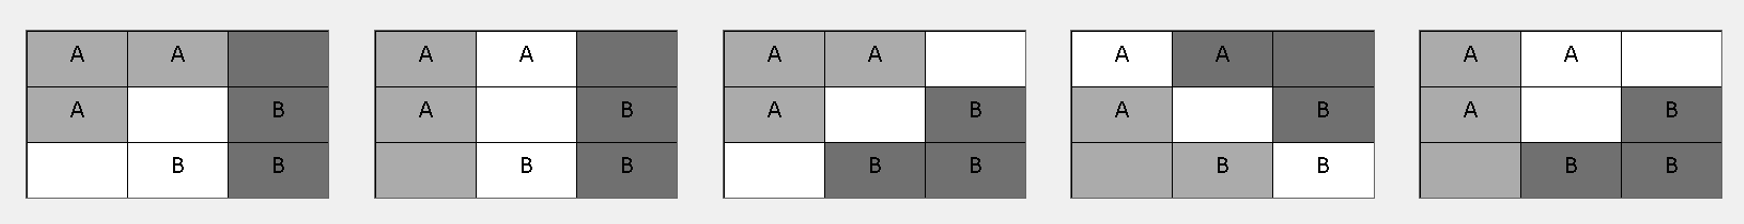
\includegraphics[scale=0.5]{maps.png}
\caption{Maps shown to participants}
\label{fig:maps}
\end{figure}
For maps 1 and 5 the configuration of these pre-determined zones provides an advantage to Player B and Player A respectively. Any zone that is not pre-determined can be thought of as being open. A subject wins an open zone with probability $\frac{e_{mi}}{e_{mi}+e_{mj}}$ where $e_{mi}$ is the effort/bid chosen by player $i \in \{1,2\}$ in map $m\in \{1,2,3,4,5\}$ for $i \not= j$. To win a district a subject must win 2/3 of the zones in that district and to win a map a subject must win 2/3 the districts of that map. Subjects are paid for the outcome of a randomly chosen round. It is worth noting that total bids for any given map may not exceed 80 lab dollars, the contest prize. 
  For each round in Stage 1 (the first 10 potentially paid rounds) a map is chosen at random and the outcome of that map determines the subjects' potential payoff for that round. This ensures subjects have proper incentive to make thoughtful decisions for each map. For the next three rounds (Stage 2) subjects are also asked for their map preference. In other words, subjects identify on which map they would like to compete, enabling us to identify whether participants gerrymander when given the opportunity. In Stage 2 a map is chosen at random from the map selections of paired subjects in order to maintain incentive for thoughtful decisions on every map, not just the one chosen by the relevant subject. For the final round (Stage 3) subjects are told that their player type, A or B, is not yet determined, but that they must pick which map they would like to compete on nonetheless. After subjects make their map choice they are assigned to either Player A or Player B and must choose efforts with this knowledge. The stage then proceeds as Stage 2. For each Stage, after map selections and bids are made the results of the contest for each map are displayed with the randomly chosen map highlighted to showcase which map could determine the subjects' earnings. The information shown to subjects includes their bids for every district in every map, their opponent's bids in every district in every map, their probability of winning any given district, their probability of wining the map, and their payoff for each map.
  \end{document}
